\documentclass[12pt,a4paper]{amsart}

% ukazi za delo s slovenscino -- izberi kodiranje, ki ti ustreza
\usepackage[utf8]{inputenc}
\usepackage[T1]{fontenc}
\usepackage[slovene]{babel}
\usepackage{lmodern} 
%\usepackage[T1]{fontenc}
%\usepackage[utf8]{inputenc}
\usepackage{amsmath,amssymb,amsfonts}
\usepackage{url}
%\usepackage[normalem]{ulem}
\usepackage[dvipsnames,usenames]{color}
\usepackage{eurosym}
\usepackage{nicefrac}
\usepackage{color}
\usepackage{hyperref}
\hypersetup{
    colorlinks=true, %set true if you want colored links
    linktoc=all,     %set to all if you want both sections and subsections linked
    linkcolor=black,  %choose some color if you want links to stand out
}

\usepackage{mathtools}
\usepackage{tikz}
\usepackage{pgfplots}
% ne spreminjaj podatkov, ki vplivajo na obliko strani
\textwidth 15cm
\textheight 24cm
\oddsidemargin.5cm
\evensidemargin.5cm
\topmargin-5mm
\addtolength{\footskip}{10pt}
\pagestyle{plain}
\overfullrule=15pt % oznaci predlogo vrstico


% ukazi za matematicna okolja
\theoremstyle{definition} % tekst napisan pokoncno
\newtheorem{definicija}{Definicija}[section]
\newtheorem{primer}[definicija]{Primer}
\newtheorem{opomba}[definicija]{Opomba}

\renewcommand\endprimer{\hfill$\diamondsuit$}


\theoremstyle{plain} % tekst napisan posevno
\newtheorem{lema}[definicija]{Lema}
\newtheorem{izrek}[definicija]{Izrek}
\newtheorem{trditev}[definicija]{Trditev}
\newtheorem{posledica}[definicija]{Posledica}


% za stevilske mnozice uporabi naslednje simbole
\newcommand{\R}{\mathbb R}
\newcommand{\N}{\mathbb N}
\newcommand{\Z}{\mathbb Z}
\newcommand{\C}{\mathbb C}
\newcommand{\Q}{\mathbb Q}


% ukaz za slovarsko geslo
\newlength{\odstavek}
\setlength{\odstavek}{\parindent}
\newcommand{\geslo}[2]{\noindent\textbf{#1}\hspace*{3mm}\hangindent=\parindent\hangafter=1 #2}


% naslednje ukaze ustrezno popravi
\newcommand{\program}{Finančna matematika} % ime studijskega programa: Matematika/Finan"cna matematika
\newcommand{\imeavtorja}{Mitja Mandić} % ime avtorja
\newcommand{\imementorja}{izred.~prof.~dr. Jaka Smrekar} % akademski naziv in ime mentorja
\newcommand{\naslovdela}{Iterativne numerične metode v posplošenih linearnih modelih}
\newcommand{\letnica}{2021} %letnica diplome


% vstavi svoje definicije ...




\begin{document}

% od tod do povzetka ne spreminjaj nicesar
\thispagestyle{empty}
\noindent{\large
UNIVERZA V LJUBLJANI\\[1mm]
FAKULTETA ZA MATEMATIKO IN FIZIKO\\[5mm]
\program\ -- 1.~stopnja}
\vfill

\begin{center}{\large
\imeavtorja\\[2mm]
{\bf \naslovdela}\\[10mm]
Delo diplomskega seminarja\\[1cm]
Mentor: \imementorja}
\end{center}
\vfill

\noindent{\large
Ljubljana, \letnica}
\pagebreak

\thispagestyle{empty}
\tableofcontents
\pagebreak

\thispagestyle{empty}
\begin{center}
{\bf \naslovdela}\\[3mm]

{\sc Povzetek}
\end{center}
% tekst povzetka v slovenscini
V povzetku na kratko opi"si vsebinske rezultate dela. Sem ne sodi razlaga organizacije dela -- v katerem poglavju/razdelku je kaj, pa"c pa le opis vsebine.
\vfill
\begin{center}
{\bf Iterative numerical methods in generalized linear models}\\[3mm] % prevod slovenskega naslova dela
{\sc Abstract}
\end{center}
% tekst povzetka v anglescini


\vfill\noindent
{\bf Math. Subj. Class. (2010):} navedi vsaj eno klasifikacijsko oznako -- dostopne so na \url{www.ams.org/mathscinet/msc/msc2010.html}  \\[1mm]
{\bf Klju"cne besede:} navedi nekaj klju"cnih pojmov, ki nastopajo v delu  \\[1mm]
{\bf Keywords:} angle"ski prevod klju"cnih besed
\pagebreak



% tu se zacne besedilo seminarja
\section{Uvod}
Posplošeni linearni modeli so ključen del statistične analize. Pomagajo nam bolje razumeti relacije med rezultati meritev in s temi izsledki
predvideti trende v prihodnosti. Modeli morajo biti kar se da enostavni, ampak hkrati zagotavljati določeno natančnost. Vsa teorija nam pa v praksi
ne koristi, če konkretnih številk ne znamo izračunati.

V dobi ogromne množice podatkov je računska učinkovitost ključni del obdelave. Tu nam pomagajo numerične metode.

V delu bom najprej predstavil posplošene linearne modele in najpriljubljenejše numerične metode, ki se uporabljajo za njihovo obdelavo. 
Teorijo bom osvetlil tudi s praktičnimi primeri.

\section{Posplošeni linearni modeli}

\subsection{Sestavni deli posplošenega linearnega modela}
Vsak posplošeni linearni model sestavljajo trije deli: \textit{slučajni del} je slučajna spremenljivka $Y$ in njena porazdelitev, 
\textit{sistematični del} predstavlja relacijo med pojasnjevalnimi spremenljivkami, \textit{povezovalna funkcija} pa transformira $Y$, da se ta
bolje prilega podatkom.

\subsubsection{Slučajni del}
\textit{Slučajni del} privzame porazdelitev slučajnega vektorja $Y$, pri čemer privzemamo tudi neodvisnost komponent. Porazdelitev $Y$
privzemamo odvisno od podatkov; mnogokrat je ,,binarna``, torej ima dve možni vrednosti - ,,uspeh`` ali ,,neuspeh``. Splošneje je lahko izid tudi 
število uspehov v fiksnem številu poskusov. V takih primerih privzamemo binomsko porazdelitev. $Y$ nam lahko meri tudi števne podatke, naprimer 
koliko zabav je obiskal študent v preteklem mesecu. Seveda pa lahko $Y$ predstavlja tudi zvezne podatke,
v tem primeru lahko privzamemo normalno porazdelitev (ali pa kakšno drugo zvezno porazdelitev).
\subsubsection{Sistematični del} 
\textit{Sistematična komponenta} posplošenega linearnega modela poda relacije med pojasnjevalnimi spremenljivkami $x_{i,j}$. Te nastopajo 
linearno, torej je sistematični del enak
\[
\beta_{0} + x_{i,1}\beta_{1} + x_{i,2}\beta_{2} + \ldots + x_{i,p}\beta_{p}
\]
\subsubsection{Povezovalna funkcija}
Tretji del posplošenega linearnega modela je \textit{povezovalna funkcija}, ta nam poda funkcijo $g(\cdot)$ med slučajno komponento
in sistematičnim delom. Če označimo $\mu = E(Y)$, je
\[
    g(\mu) = \beta_{0} + x_{i,1}\beta_{1} + x_{i,2}\beta_{2} + \ldots + x_{i,p}\beta_{p}
\]
Najenostavnejša taka funkcija je kar identiteta, torej $g(\mu) = \mu$. Ta nam torej da linearno povezavo med pojasnjevalnimi spremenljivkami 
in pričakovano vrednostjo naših slučajnih spremenljivki. To je ena od oblik regresije za zvezne podatke.
Mnogokrat pa linearna relacija ni primerna - fiksna sprememba pojasnjevalnih spremenljivk ima lahko večji vpliv, če je pričakovana vrednost 
bližje 0, kot če je bližje 1. Recimo, da je $\pi$ verjetnost, da bo oseba kupila nov avto, ko je njen dohodek enak $x$. Sprememba v dohodku
za 10.000\euro~ima manjši vpliv, če je dohodek 1.000.000\euro,~kot če je 50.000\euro.
Takrat je smiselno uporabiti kakšno drugo povezovalno funkcijo, ki dopušča tudi nelinearne kombinacije pojasnjevalnih
spremenljivk. Naprimer, $g(\mu) = \log(\mu)$ modelira
pričakovano vrednost logaritma. Smiselno jo je uporabiti, če pričakovana vrednost ne more zavzeti negativnih vrednosti. Takemu modelu rečemo
\textit{log-linearen} model.
Spet druga povezovalna funkcija je $\mathrm{logit}(\mu) = \log(\frac{\mu}{1-\mu})$, ki nam modelira logaritem deležev - smiselno jo je uporabiti, 
ko $\mu$ ne zavzame vrednosti izven $(0,1)$, torej ko imamo opravka z verjetnostmi. Takemu modelu rečemo logistični model.
%\subsection{Primeri posplošenih linearnih modelov}
\subsection{Točkovno ocenjevanje}
Preden se natančneje posvetimo posplošenim linearnim modelom, si oglejmo dve najbolj znani metodi za ocenjevanje parametrov.

\subsubsection{Metoda momentov}
Metodo momentov Čebišev je leta 1887 predstavil v svojem dokazu centralnega limitnega izreka.

\subsubsection{Metoda največjega verjetja}
\subsection{Linearna regresija}
Linearna regresija je najenostavnejši primer posplošenega linearnega modela. Enostavno jo lahko zapišemo kot:
$
    Y = X \beta + \varepsilon
$
kjer je $Y$ proučevan slučajni vektor, $X$ je matrika pojasnjevalnih slučajnih spremenljivk, $\beta$ je vektor koeficientov, ki jih želimo oceniti,
$\varepsilon$ pa slučajna spremenljivka, ki predstavlja napako - pri računanju, meritvah \ldots. Privzemimo, da je $E(\varepsilon) = 0$. Iz tega sledi
$\mu = E(Y) = X\beta$. Model torej pričakovano vrednost slučajne spremenljivke predstavi kot linearno funkcijo pojasnjevalnih spremenljivk.
Parametre $\beta$ ocenimo z metodo najmanjših kvadratov in ob predpostavki polnega ranga za matriko $X$ dobimo $\hat{\beta} =  (X^\top X)^{-1}
X^\top Y$. 
\subsection{Poissonova regresija}
\subsection{Logistična regresija}
Logistična regresija se uporablja za določanje deležev oziroma računanje verjetnosti. V poštev pride, ko imamo odgovore tipa uspeh-neuspeh oziroma
govorimo o prisotnosti ali odsotnosti neke lastnosti.
Spomnimo se Binomske porazdelitve $Y_{i} \sim B(n_{i}, p_{i})$. Ta pravi, da je 
\[
    P(Y_{i} = y_{i}) = {n_{i} \choose y_{i}} p_{i}^{y_{i}}(1 - p_{i}) ^{n_{i} - y_{i}}
\]
Pričakovana vrednost in varianca sta odvisni le od $p_{i}$, in sta enaki $E(Y_{i}) = n_{i}p_{i} \text{~in}\\Var(Y_{i}) = n_{i}p_{i}(1 - p_{i}).$~
Poglejmo si sedaj podrobneje \textit{logit} transformacijo. Če se spomnemo, želimo določiti verjetnost nekega dogodka pri danih podatkih. Ob uporabi
identitente transformacije se nam kaj hitro lahko zgodi, da za posamezne verjetnosti dobimo vrednosti izven intervala $[0,1]$. Ta problem bomo rešili v 
dveh korakih.
Najprej uvedimo 
\[ 
    \mathrm{delez}_{i} = \frac{p_{i}}{1 - p_{i}} %poglej kako se tle da vejico
\]
kjer se premaknemo iz verjetnosti v \textit{deleže} -- verjetnost dogodka proti verjetnosti, da se ne bo zgodil. Če je $p_{i}$ enak $\frac{1}{2}$, 
bo delež enak 1. Vidimo, da so deleži vedno pozitivni in niso omejeni navzgor.
V naslednjem koraku pa poglejmo logaritem deležev ali logit verjetnosti
\[
    \eta_{i} = \mathrm{logit}(p_{i}) = \log \frac{p_{i}}{1 - p_{i}}
\]
s tem pa si odstranimo tudi omejitev navzdol. Opazimo še, da če je $p_{i} = \frac{1}{2}$, je delež enak 1 in je logaritem 0. Kot funkcija p, je logit
strogo naraščajoča, torej imamo inverz. Običajno ga imenujemo \textit{antilogit}, izrazimo ga z:
\[
    p_{i} = \mathrm{logit}^{-1}(\eta_{i}) = \frac{\exp{\eta_{i}}}{1+\exp{\eta_{i}}} = \frac{\exp{x_{i}^\top\beta}}{1+\exp{x_{i}^\top\beta}}
\]
Vse skupaj nam da \textit{logistični model}, ki za slučajni del vzame binomsko porazdelitev. %VPRAŠAJ KAJ JE Z NAPAKO
Kot vidimo, zveza med prediktorji in verjetnostjo ni linearna, zato je težko oceniti, kako bo sprememba parametrov
vplivala na verjetnost. Na to vprašanje lahko približno odgovorimo tako, da odvajamo po spremenljivki $x_{j}$ (kar ima seveda smisel le za zvezne
pojasnjevalne spremenljivke) in dobimo $\nicefrac{\partial}{\partial x_{j}} = \beta_{j}p_{i}(1 - p_{i}).$~Vidimo, da na spremembo j-tega prediktorja
vpliva tako verjetnost kot tudi parameter $\beta$. Običajno se za analizo vzame vzorčno povprečje verjetnosti opazovane vrednosti.
\subsubsection{Ocenjevanje parametrov}\label{ocenpar}
Imamo binomske slučajne spremenljivke in imamo povezovalno funkcijo, $\mathrm{}{logit p_{i}} = X\beta$, kjer so $\beta$ neznani parametri.
V naslednjem razdelku si bomo ogledali kako zanje izpeljemo enačbe verjetja, ki jih nato uporabimo v numeričnih algoritmih.
Kot v vsakem posplošenem linearnem modelu tudi v tem predpostavimo neodvisnost komponent slučajnega vektorja $\mathrm{Y}$ zato 
\begin{align*}
    P(Y = \vec{y}) &= \prod_{i=1}^{n} P(Y_{i} = y_{i}) \\
                    &=\prod_{i=1}^{n} {n_{i} \choose y_{i}} p_{i}^{y_{i}}(1 - p_{i})^{n_{i} - y_{i}}
\end{align*}
Naprej si oglejmo logaritemsko funkcijo verjetja. V nadaljnem računanju bom izpuščal binomski simbol na začetku - je samo konstanta, ki na
končen rezultat nima vpliva. Po prejšnjih oznakah je torej
\begin{align}\label{logit1}
    \ell(p_{i}) &= \log\{\prod_{i=1}^{n} p_{i}^{y_{i}}(1 - p_{i})^{n_{i} - y_{i}} \} \nonumber  \\
        &= \sum_{i=1}^{n}\{y_{i}\log{p_{i}} + (n_{i} - y_{i})\log(1 - p_{i})\} \nonumber \\
        &= \sum_{i=1}^{n}\{n_{i}\log{1-p_{i}}  + y_{i}\log{\left(\frac{p_{i}}{1-p_{i}}\right)}\}
\end{align}
Po predpostavki logističnega modela je 
\[
   \mathrm{logit}(p_{i}) = \log\left( \frac{p_{i}}{1-p_{i}}  \right) = \beta_{0} + x_{i1}\beta_{1} + \ldots + x_{ir}\beta_{r} = x_{i}^\top \beta,
\]
iz česar lahko izrazimo verjetnost $p_{i}$
\begin{align}
    p_{i} &= \frac{\exp{x_{i}^{\top} \beta}}{1 + \exp{x_{i}^\top\beta}} \text{~ter} \\
    1 - p_{i} &= \frac{1}{1 + \exp{x_{i}^\top\beta}}
\end{align}

\pagebreak
Zgornji funkciji rečemo \textit{sigmoida}. Iz njenega grafa je morda še bolj očitno, zakaj jo je smiselno uporabiti za modeliranje verjetnosti
\begin{center}
\begin{figure}[h]
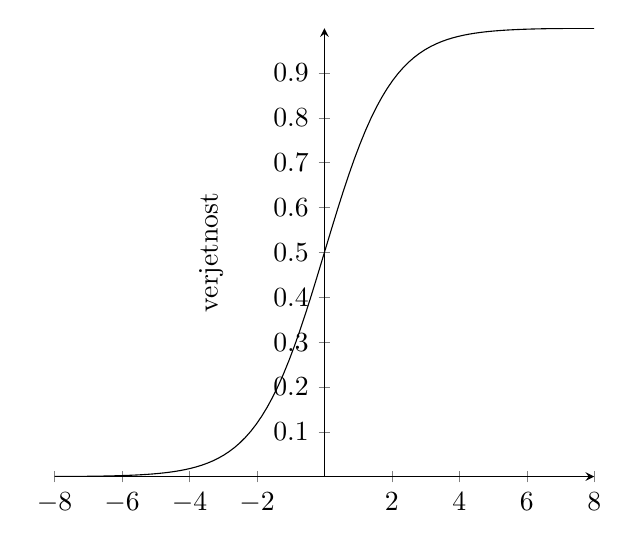
\begin{tikzpicture}
    \begin{axis}[
        axis lines = center,
        %xtick = {-10,-9,-8,...,9,10}
        ytick = {0,0.1,0.2,...,0.9,1},
        ylabel = verjetnost,
        y label style = {at={(axis description cs:0.25,.5)},rotate=90}%,anchor=south}
    ]
    \addplot [
        domain=-8:8, 
        samples=100, 
        color=black,
        ]
        {exp(x)/(1+exp(x))};
    %\addlegendentry{$x^2 + 2x + 1$}
    
    \end{axis}
\end{tikzpicture}
\caption{Graf sigmoide}
\label{fig:sigmoid}
\end{figure}
\end{center}

Če izpeljane izraze za verjetnost upoštevamo v logaritemski funkciji verjetja dobimo
\begin{align}
    \ell(\beta) &= \sum_{i=1}^{n}\left( n_{i}\log{\frac{1}{1 + \exp{x_{i}^\top\beta}}}  + y_{i}\log{\left( \frac{\frac{\exp{x_{i}^{\top} \beta}}{1 + \exp{x_{i}^\top\beta}}}{\frac{1}{1 + \exp{x_{i}^\top\beta}}}  \right)} \right) \nonumber\\
                &= \sum_{i=1}^{n}\left( y_{i}(x_{i}^\top\beta) - n_{i}\log(1 + \exp{x_{i}^\top\beta})           \right)
\end{align}
Od tod vidimo, da je naša funkcija verjetja zares odvisna le od parametrov $\beta$,~vse ostalo nam je poznano. Da torej poiščemo maksimum in s tem
cenilko največjega verjetja, funkcijo odvajamo in zbirno funkcijo enačimo z 0
\[
    \dot{\ell}(\beta) = \begin{bmatrix}
                                 \frac{\partial \ell(\beta)}{\partial \beta_{0}} \\
                                 \frac{\partial \ell(\beta)}{\partial \beta_{1}} \\
                                 \vdots \\
                                 \frac{\partial \ell(\beta)}{\partial \beta_{p}}
                        \end{bmatrix}
\]
Pomembno je opaziti, da parametri $\beta$ vedno nastopajo ob pojasnjevalnih spremenljivkah linearno -- zato bodo komponente zbirne funkcije simetrične.
J-ta komponenta bo tako enaka
\begin{align}
    \frac{\partial \ell(\beta)}{\partial \beta_{j}} &= \sum_{i=1}^{n} \left(x_{ij}(y_{i} - n_{i}p_{i}(\beta))   \right),~~j = 0,1,\ldots r, \text~~{kjer smo upoštevali} \\
    \frac{\partial}{\partial \beta_{j}}(x_{i}^\top\beta) &= \frac{\partial}{\partial \beta_{j}}\left(\beta_{0} + x_{i1}\beta_{1} + \ldots x_{ir}\beta_{r}\right) \nonumber\\
                                                    &= x_{ij} \text{ter} \\    
    \frac{\partial}{\partial \beta_{j}} \log(1 + \exp(x_{i}^\top\beta)) &= \frac{ \frac{\partial}{\partial \beta_{j}}\exp(x_{i}^\top\beta) }{1 + \exp(x_{i}^\top\beta)} \nonumber \\
    &= \frac{\exp(x_{i}^\top\beta)}{1 + \exp(x_{i}^\top\beta)} \frac{\partial}{\partial \beta_{j}} (x_{i}^\top\beta) \nonumber \\
    &=p_{i}(\beta)x_{ij}
\end{align}
Enačbe, ki jih s tem postopkom dobimo, v splošnem niso eksplicitno rešljive. Za reševanje se uporablja numerične metode, ki pa slonijo na Newtonovi iteraciji.
Zanjo pa je potrebno izračunati še drugi odvod, zato to storimo tu. Zopet odvajamo po komponentah, tako kot zgoraj. Najprej izračunajmo
\begin{align}
    \frac{\partial p_{i}(\beta)}{\partial \beta_{k}} &= \frac{\partial}{\partial \beta_{k}} \frac{\exp{x_{i}^\top\beta}}{1+\exp{x_{i}^\top\beta}} \nonumber \\
        &= x_{ik}p_{i}(\beta)(1 - p_{i}(\beta)) \nonumber
\end{align}
Vse sedaj skupaj sestavimo v
\begin{align}
    \frac{\partial^2}{\partial \beta_{j}\partial\beta_{k}} = - \sum_{i}^{n}\left(x_{ij}x_{ik}n_{i}p_{i}(\beta)(1-p_{i}(\beta))\right),~~j,k = 0,1,\ldots, r
\end{align}
Spomnimo se, da delamo z binomskimi slučajnimi spremenljivkami in torej velja $var(Y_{i}) = v_{i}(\beta) = n_{i}p_{i}(1-p_{i}),$~kar vključimo v zgornjo enačbo in končno dobimo
\begin{align}
    \ddot{\ell}(\beta) = -\sum_{i=1}^{n}\left(x_{ij}x_{ik}v_{i}(\beta)\right).
\end{align}
Zapišimo zgoraj izpeljane zveze v berljivejšo matrično notacijo. 
\begin{equation*}
    \log \left(\frac{p}{1-p}\right) = \mathbf{X}\beta
\end{equation*}
Vektorsko definiramu tudi
\[
    \exp{\mathbf{X}\beta} = \begin{bmatrix}
                            \exp{x_{1}^\top\beta} \\
                            \vdots\\
                            \exp{x_{n}^\top\beta}
                            \end{bmatrix},
\]
spomnimo se enačbe \eqref{logit1} in iz nje izpeljimo
\begin{align} \label{ell}
    \ell(\beta) &= \sum_{i=1}^{n}\{n_{i}\log{1-p_{i}}  + y_{i}\log{\left(\frac{p_{i}}{1-p_{i}}\right)}\} \nonumber\\
    &= y^\top\mathbf{X}\beta - n^\top \log(1 + \exp{\mathbf{X}\beta}),
\end{align}
in še odvoda zgornje funkcjie, ki pa ga lahko zapišemo kot
\begin{align}
    \dot{\ell}(\beta) = \mathbf{X}^\top(y - m\circ p(\beta)),
\end{align}
kjer je s $\circ$ označeno Hadamardovo množenje po elementih.
S pričakovano vrednostjo vektorja označimo vektor pričakovanih vrednosti komponent in torej lahko zapišemo
\begin{equation}
    \mathrm{E}(Y) = m \circ p(\beta) \equiv \mu(\beta),
\end{equation}
in lahko končno vse povzamemo v
\begin{align}\label{prvi}
    \dot{\ell}(\beta) = \mathbf{X}^\top(y - m \circ p(\beta)) = X^\top(y - \mu(\beta))
\end{align}
Ostane nam le še dvojni odvod. Najprej si oglejmo
\[
    v(\beta) = \begin{bmatrix}
        v_{1}(\beta)  & & &\\
        & v_{2}(\beta) & & \\
        & & \ddots & \\
        & & & v_{n}(\beta)
    \end{bmatrix},
\]
iz tega potem takoj sledi, da je
\begin{equation} \label{drugi}
    \ddot{\ell}(\beta) = -\mathbf{X}^\top v(\beta)\mathbf{X},
\end{equation}
torej element v $j$-ti vrstici in $k$-tem stolpcu je $\sum_{i=1}^{n}x_{ij}x_{ik}v_{i}(\beta).$

\subsection{Probit regresija}
Probit regresija se uporablja v podobne namene kot logistična, torej za določanje verjetnosti in razvrščanje. Razvili so jo v tridesetih letih
dvajsetega stoletja, ime pa je skovanka -- pride iz anglešlih besed \textit{\textbf{prob}ability un\textbf{it}}. V glavnem se od logistične regresije
razlikuje v sistematičnem delu. Verjetnost pozitivnega izida torej po modelu predpostavljamo
\begin{equation}
    p_{i}(\beta) = \Phi (\beta_{0} + x_{i1}\beta_{1} + \ldots + x_{ir}\beta_{r}),
\end{equation}
kjer $\Phi$ predstavlja kumulativno porazdelitveno funkcijo standardne normalne slučajne spremenljivke. Ta seveda ni linearna, ne znamo je niti zapisati z 
elementarnimi funkcijami. Podobno kot v logističnem modelu, se bomo ocenjevanja parametrov lotili po metodi največjega verjetja.

\subsubsection{Ocenjevanje parametrov probit regresije}


\section{Numerične metode}
V sledečih razdelkih si bomo od bliže pogledali nekaj numeričnih metod, uporabljenih v kasnejših zgledih. Te metode slonijo na stoletja starih
idejah, ki smo jih spoznali tekom študija, uporabljajo pa se tudi v številnih praktičnih aplikacijah.
\subsection{Newton -- Raphsonova metoda} \label{nr}
Newton -- Raphson (oziroma le Newtonova) metoda je bila v osnovi razvita za iskanje ničel funkcije. V najosnovnejši (ter najpogostejši) verziji za iskanje
ničle funkcije ene spremenljivke začnemo v neki točki, naslendnjo pa izberemo v presčišču tangente, izračunane v 
tej točki, z x-osjo. Postopek tako iterativno nadaljujemo. Ideja je torej sila preprosta, za izpeljavo pa tudi ni potrebno preveč truda.
Predpostavimo odvedljivost funkcije na nekem intervalu in recimo, da imamo trenuten približek $x_{n}.$~Razvijmo sedaj funkcijo v Taylorjev
polinom prve stopnje okoli $x_{n}:$
\[
    f(x) \approx f(x_{n}) + f'(x_{n})(x - x_{n})
\]
Presečišče najdemo, če zgornjo enačbo enačimo z 0 in dobimo znano formulo
\[
    x_{n+1} = x_{n} - \frac{f(x_{n})}{f'(x_{n})}.
\]
Metoda bo skonvergirala za začetne približke dovolj blizu ničli in v neki okolici ničle konvergirala s kvadratično hitrostjo. 
Na težave naletimo v več primerih. Najprej, blizu stacionarne točke metoda odpove, saj bi delili z 0 (oziroma vrednostmi blizu ničle, kar je numerično nestabilno).
Problem lahko predstavlja tudi računanje odvoda, ki zna biti zahtevno, ter dejstvo, da za slabe začetne približke ničle morda ne bomo našli. S temi 
težavami se bomo soočili v nadaljevanju.
Imamo torej algoritem, ki najde ničlo, v luči iskanja cenilke največjega verjetja pa bi želeli algoritem, ki poišče maksimum oziroma minimum funkcije.
Recimo, da imamo neko logaritemsko funkcijo verjetja $L$, in trenutni približek $\theta_{n}$. Razvijmo funkcijo okoli približka v Taylorjev polinom
druge stopnje:
\begin{align}
    L(\theta) \approx L(\theta_{n}) + dL(\theta_{n})(\theta - \theta_{n}) + \frac{1}{2}(\theta - \theta_{n})^\top d^{2}L(\theta_{n})(\theta - \theta_{n}) \label{taylor}   
\end{align}
Maksimizirati želimo desno stran \eqref{taylor}. To storimo tako, da gradient $L$ enačimo z nič:
\[
    \nabla L(\theta_{n}) + \nabla^2L(\theta_{n})(\theta - \theta_{n}) = 0  
\]
in izrazimo naslednji približek
\[
    \theta_{n + 1} = \theta_{n} - \nabla^{2}L(\theta_{n})^{-1}\nabla L(\theta_{n}).
\]
S tem postopkom imamo lahko dva problema. Prvič, lahko je zahtevno računati in invertirati drugi odvod (Hesian) funkcije, morda za kakšen $\theta_{n}$ sploh ne obstaja.
Drugič, proč od $\hat{\theta}$ lahko Newtonova metoda napreduje navzgor ali navzdol -- oboje je enako verjetno. Z drugimi besedami, Newtonova metoda ni naraščajoč algoritem in torej
ne da $L(\theta_{n}) < L(\theta_{n+1}).$ Mi pa bi želeli algoritem, ki bo konvergiral globalno (in ne le na nekem intervalu okoli rešitve).
Težavo z računanjem inverza rešimo tako, da namesto invertiranja problem prevedemo na reševanje sistema enačb za premik:
\begin{align}\label{newtoneq}
    x_{n + 1} &= x_{n} + p_{n} \nonumber\\
    \nabla^2L(\theta_{n})p_{n} &= -\nabla L(\theta_{n})
\end{align}
Zadnji vrstici v \eqref{newtoneq} rečemo tudi \textit{Newtonova enačba}.
Radi bi še dosegli, da bi se Newtonov algoritem premikal v eno smer, torej naraščal ali padal. S tem bi vedeli, kaj se bo zgodilo v iteraciji in lažje predvideli morebitne
nevšečnosti. Newtonova metoda za iskanje minimuma (maksimum) funkcije je optimizacijski problem drugega reda in realna funkcija ima globalni minimum (maksimum) tam, kjer je
njen drugi odvod pozitiven, oziroma v primeru funkcij več spremenljivk, kjer je njen Hesian pozitivno definiten (in je tam gradient enak nič). Če bi torej imeli
strogo pozivino definitno matriko, bi bil ta optimizacijski problem konveksen in kot tak rešljiv globalno (veljati morajo še pogoji Karush-Kuhn-Tuckerja, vendar je to skoraj vedno res).
Imejmo torej v točki $x^{*}$ pozitivno definitno Hessejevo matriko $H.$~Zapišimo Taylorjev polinom druge stopnje okoli te točke
\[
    f(x^{*} + s) = f(x_x^{*}) + \nabla f(x^{*})s + \frac{1}{2}s^\top H(x^{*})s.
\]
Če velja še pogoj prvega reda, torej $\nabla f(x^{*}) = 0,$~imamo
\[
    f(x^{*} + s) = f(x^{*}) + \frac{1}{2}s^\top H(x^{*})s,
\]
kar pomeni, da se vrednost funkcije vedno poveča, če se premaknemo iz stacionarne točke $x^{*}$~(drugi člen je vedno pozitiven zaradi pozitivne definitnosti)
Tako vidimo, da imamo strogo padajoč algoritem.
\subsection{Fisher's scoring}
Fisher's scoring algoritem je variacija v prejšnjem razdelku opisanega Newton -- Raphsonovega algoritma, ki se v statistiki uporablja za numerično reševanje enačb največjega 
verjetja. Poimenovana je po Ronaldu Fisherju, enem najpomembenjših angleških statistikov dvajsetega stoletja.
Uvedimo najprej nekaj terminologije in oznak. Kot v prejšnjih poglavijh, imamo veliko opravka logaritemsko funckijo verjetja (angl. \textit{log-likelihood function}), ki jo tu označimo 
z $L = \log \left(f(x_{1},\theta)\ldots f(x_{n},\theta) \right),$ ki jo obravnavamo kot funkcijo parametra $\theta$ pri fiksnem vzorcu. Po drugi strani pa je to
tudi transformacija porazdelitvene funkcije slučajnega vektorja $X = (X_{1},X_{2},\ldots,X_{n}),$ kjer privzamemo neodvisnost komponent (kar pa seveda velja v vseh
modelih, ki jih obravnavamo v tej nalogi). Zbirna funkcija (angl. \textit{score function}) je gradient logaritemske funkcije največjega verjetja po ocenjevanem parametru. 
Informacijska (oziroma Fisherjeva Informacijska) matrika (angl. \textit{(Fisher) information matrix}) je definirana kot 
\[
    I(\theta) = \mathrm{E}[\nabla L(\theta) \nabla L(\theta)^\top ]. %= \mathrm{E}[\dot{\ell}(\theta) \dot{\ell}(\theta)^\top].
\]
Fisher scoring algoritem sedaj je po zgornjih oznakah 
\begin{align}
    \theta{n + 1} = \theta_{n} - I(\theta)^{-1}\nabla L(\theta)
\end{align}
\subsubsection{Fisherjeva informacijska matrika in informacijska enakost}
V sledečem razdelku bomo utemeljili uporabo Fisher scoring algoritma in prikazali njegovo glavno prednost pred običajno Newtonovo iteracijo, opisano v poglavju \ref{nr}.
Ob določenih predpostavkah o gladkosti logaritemske funkcije verjetja (ki za eksponentno družino vedno držijo), bomo sedaj pokazali, da je pričakovana vrednost
zbirne funkcije enaka nič. Tu smo $\ell(\theta)$ označili z $\log f_{\theta}(x)$.
\begin{align} \label{Ezbirne}
    \mathrm{E}[\nabla L (\theta)] &= \int f_{\theta}(x) \nabla_{\theta}\log(f_{\theta}(x)) \,dx = \int f_{\theta}(x) \frac{\nabla f_{\theta}(x)}{f_{\theta}(x)} \,dx \nonumber \\
        &= \int \nabla f_{\theta}(x) \,dx \overset{*}{=} \nabla \int f_{\theta}(x) \,dx = \nabla 1 = 0, 
\end{align}
kjer smo v enakosti $(*)$ zamenjali integracijo in odvajanje, kar po teoriji mere smemo - gostota porazdelitev eksponentne družine je zvezno odvedljiva. 
Velja tudi
\[
    \nabla^{2} \log{f_{\theta}(x)} = \frac{\nabla^2 f_{\theta}(x)}{f_{\theta}(x)} - \frac{\nabla f_{\theta}(x) \nabla f_{\theta}(x)^\top }{f_{\theta}(x)^{2}} = 
    \frac{\nabla^2 f_{\theta}(x)}{f_{\theta}(x)} - \dot{\ell}(\theta)\dot{\ell}(\theta)^\top,
\]
kjer smo v zadnji enakosti upoštevali
\[
    \nabla L (\theta) = \nabla \log(f_{\theta}(x)) = \frac{\nabla f_{\theta}(x)}{f_{\theta}(x)} 
\]
Povzemimo vse, kar smo dokazali v prejšnjih enačbah in imamo
\begin{align}\label{infoeq}
    I(\theta) &= \mathrm{E}[\nabla L(\theta)(\nabla L(\theta))^\top] =  -\int f_{\theta}(x) \nabla^2 \log f_{\theta}(x) \,dx+ \int \nabla^2 f_{\theta}(x) \,dx \nonumber \\
    &= -\mathrm{E}[\nabla^2 \log f_{\theta}(x)] + \nabla^2\int \nabla^2 \log f_{\theta}(x) \,dx = -\mathrm{E}[\nabla^2 \log f_{\theta}(x)]
\end{align}
Enačbi \eqref{infoeq} rečemo tudi \textit{informacijska enakost}. To nam bo koristilo pri dokazovanju enakosti med Newton -- Raphson algoritmom in Fisher scoringom za logistični model.
Kot smo videli v prejšnjih poglavjih, želimo imeti pozitivno semi-definitno matriko in s tem monoton algoritem. Izkaže se, da je informacijska matrika ravno variančno-kovariančna matrika
zbirne funkcije. Po enačbi \eqref{Ezbirne} se spomnimo, da je pričakovana vrednost zbirne funckije enaka 0. Potem takoj sledi
\begin{align}
    I(\theta) &= \mathrm{E}[\nabla L(\theta)\nabla L(\theta)^\top] \nonumber\\
    &= \mathrm{E}[\left(\nabla L(\theta) - \mathrm{E}[\nabla L(\theta)]\right)\left(\nabla L(\theta) - \mathrm{E}[\nabla L(\theta)]\right)^\top] \nonumber \\
    &= \mathrm{Var}[\nabla L(\theta)].
\end{align}
Variančno-kovariančne matrike pa so pozitivno semi-definitne.
\subsubsection{Fisher's scoring v logističnem modelu}
Poglejmo za trenutek nazaj v poglavje \ref{ocenpar}, natančneje k enačbam \eqref{ell},\eqref{prvi} in \eqref{drugi}. Iz prejšnjega razdelka vemo tudi, da velja
\[
    I(\theta) = \mathrm{E}[-\nabla ^2 L(\theta)] \overset{\eqref{drugi}}{=} X^\top v(\theta)X = -\nabla ^2 L(\theta),
\]
kjer smo seveda uporabili tudi prej dokazano informacijsko enakost. Tako vidimo, da Fisher's scoring in Newton--Raphsonova metoda v primeru logistične regresije
res sovpadata, saj je matrika drugih odvodov ravno enaka informacijski matriki. Če zapišemo sedaj vse skupaj
\begin{align}
    \hat{\theta}_{i+1} &= \hat{\theta}_{i} - (\nabla^{2} L(\hat{\theta}_{i}))^{-1} \nabla L(\hat{\theta}_{i}) \nonumber \\
    &= \hat{\theta}_{i} + (\mathbf{X}^\top v(\hat{\theta}_{i}) \mathbf{X})^{-1}\mathbf{X}^\top(y - \mu(\hat{\theta}_{i})) 
\end{align}
\section{Primeri}
\subsection{Ocenjevanje parametrov v logističnem modelu}

V praktično usmerjenem delu te naloge smo v Pythonu implementirali zgoraj opisani postopek Fisher scoring algoritma za binomsko porazdeljene slučajne
spremenljivke. Za delo v Pythonu smo uporabili več knjižnic\; \texttt{NumPy} za računanje z matrikami in vektorji, reševanje sistemov enačb ter invertiranje,
knjižnico \texttt{pandas} za uvoz podatkov in njihovo začetno urejanje. Na koncu smo si s paketom \texttt{Pyplot} iz knjižnice \texttt{Matplotlib} rezultate izrisali.
V implementaciji smo popolnoma sledili zgoraj izpeljanim enačbam, zato jih tu nebomo ponovno navajali.
\subsection{Ocenjevanje parametrov v probit modelu}
% slovar
\section*{Slovar strokovnih izrazov}
%\geslo{}{}
%
%\geslo{}{}
%
% seznam uporabljene literature
%\begin{thebibliography}{99}
%\bibitem{}
%end{thebibliography}
\nocite{*}
\bibliographystyle{plain}
\bibliography{literatura}
\end{document}
